\chapter{Introduction}

Moving meshes are required in various problems in computational fluid dynamics (CFD), such as fluid-structure interaction, aerodynamic shape optimization \cite{appl:opt, appl:mavriplis} and some kinds of multi-material flow simulations. Mesh movement may also be used in generating curved meshes for spatially high-order computational methods \cite{curve:persson}. 

In fluid-structure interaction, the boundaries shared by the solid and fluid domains need to move according to the deformation of the solid, so that the response of the fluid to that movement can be captured. Thus for a body-fitted mesh, robust mesh movement is needed, though it must be mentioned that immersed boundary methods can also be used for fluid structure interaction, in which the mesh is no longer fitted to the fluid-structure boundary. Both methods have their advantages and disadvantages \cite{appl:fsireview}. Mesh movement could be used to enable this \cite{mm:fsielast}. In shape optimization, the geometry needs to change after each design cycle, and a good mesh movement method is usually necessary \cite{appl:opt}. Mesh movement could also be used to track discontinuities in multi-material simulations.

In general, good properties of a mesh movement scheme are as follows.
\begin{enumerate}
\item It should be robust. In many kinds of meshes, such as meshes required for viscous flow computations, even small boundary movements can invalidate the mesh. The scheme should be able to preserve mesh validity, at the very least.
\item Mesh quality should be preserved to a great extent. Elements should not become highly skewed or mis-shaped after movement, as this can impact flow computations on the deformed mesh. We discuss skew and shape of elements later in the report.
\item It should be computationally inexpensive. Many applications need very fast mesh movement schemes as they require the mesh to be moved many times during the simulation, possibly every time step.
\end{enumerate}
Some mesh movement schemes that we present here satisfy only one or two of the above criteria. Our aim is to find a scheme that satisfies all three criteria well. We give a review of various mesh-movement methods in chapter 2. While the method of non-linear elasticity \cite{curve:persson} is very robust, it is also very expensive. Thus we consider linear elasticity based methods and several methods of the interpolation type as our main candidates. The latter methods involve interpolation of boundary displacements to the interior using various techniques; we find that these tend to be computationally much less explensive than elasticity-based methods. Some of them give results similar to linear elasticity methods while taking significantly less computational time; we demonstrate this in the results (chapter 4).

High-order computational methods are becoming popular in the aerospace community in recent years. Research is being conducted in robust high-order schemes that work on unstructured/hybrid grids, including continuous finite element methods such as streamline-upwind Petrov Galerkin methods \cite{appl:supg}, discontinuous Galerkin finite element methods \cite{solver, curve:hartmann, appl:mavriplis}, spectral element methods \cite{appl:spectral}, flux reconstruction \cite{appl:fr} and high-order finite volume methods, among others. According to Wang, Fidkowski \emph{et. al.}, high-order methods are better than prevailing second-order methods for smooth flows. While conclusive data was not available for flows with discontinuities, high-order methods with \emph{hp} adaptation might outperform second-order methods. One of the areas facing challenges, according to them, is high-order mesh generation \cite{highorder}. 

High-order approximation of the boundary is required to attain high-order spatial accuracy \cite{curve:geomacc}, and in some cases it may be crucial to even preserve qualitative correctness of the flow. For example, if high-order boundary representation is not used with a DG P1 (discontinuous Galerkin with piecewise linear basis functions) scheme, the solution to the 2D Euler equations around a cylinder shows a wake and vortex shedding \cite{appl:dgeuler} (figure \ref{fig:bassi}).
 \begin{figure}[!h]
 	\centering
 	\subfloat{
 		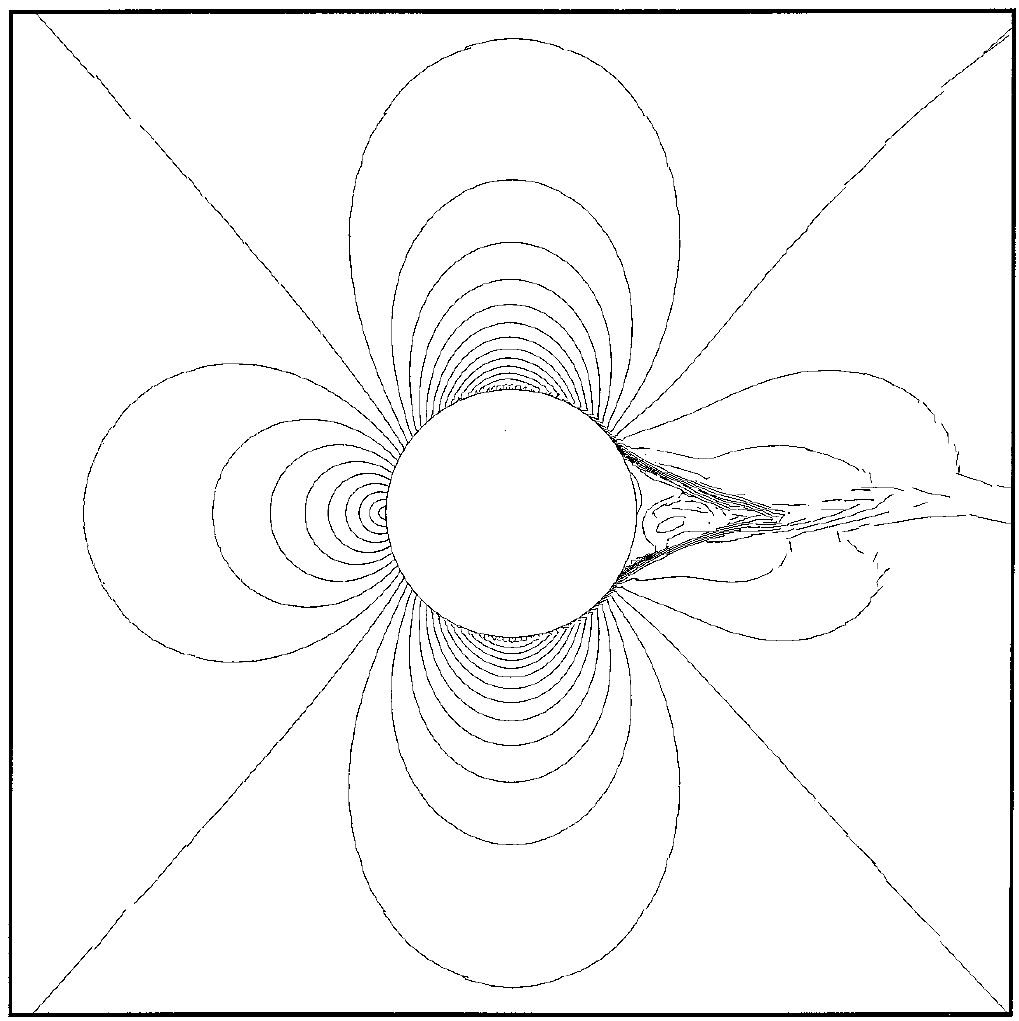
\includegraphics[scale=0.15]{bassi-linear}
 	}
 	\subfloat{
 		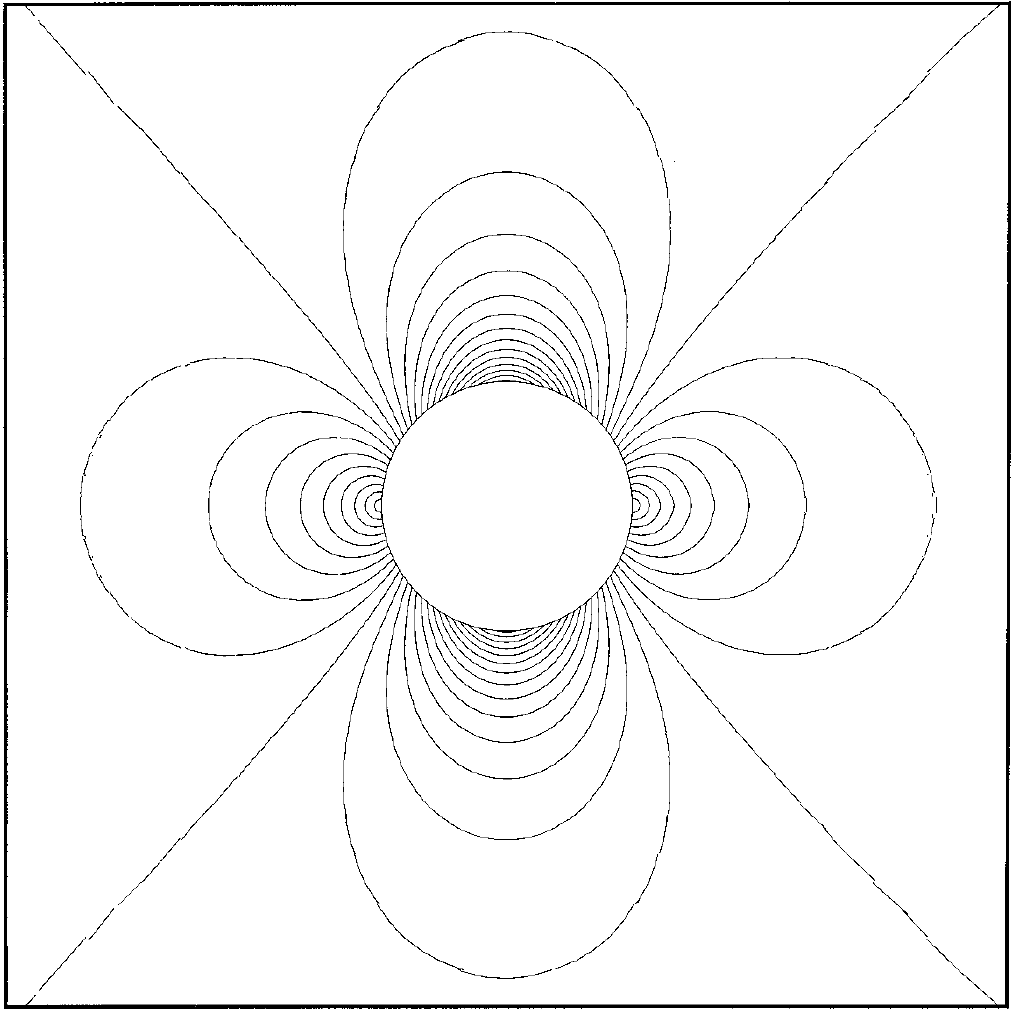
\includegraphics[scale=0.15]{bassi-q2}
 	}
 	\caption{Inviscid subsonic flow over a cylinder; left: DGP1 solution with regular linear mesh, right: DGP1 solution with quadratic (`Q2') mesh \cite{appl:dgeuler}}
 	\label{fig:bassi}
 \end{figure}
Thus, robust techniques to obtain a high-order representation of the geometry (the boundary of the domain) have become important.  One technique of high-order boundary approximation is to produce high-order meshes, otherwise called curved meshes. Another technique in this regard is isogeometric analysis \cite{isogeometric} where CAD data is directly used in analysis. In this work, we deal with curved unstructured mesh generation, using either CAD data if available, or only the linear mesh data. If only linear mesh data is available, a high-order boundary reconstruction is used to compute a higher order approximation, and the mesh is then curved according to this reconstructed boundary. Once the boundary is curved, regularization of the interior mesh is generally required to maintain mesh quality.

In chapter 3, the method of curved mesh generation adopted for this work is described. For regularizing the interior mesh, we prefer interpolation by radial basis functions (RBF) \cite{rbf:errorwendland}. We compare this method with the `stiffened' linear elasticity method \cite{mm:fsielast}. For our test cases, both are found to work quite well but the RBF method takes comparatively very little time.

Results for both mesh movement and curved mesh generation are presented in chapter 4. We conclude in chapter 5 with a comparison of the methods, and give some more details of our implementation in the appendices.
